 \section{Predictability, Complexity, and Permutation Entropy %{\color{blue}  EDITABLE}
 } % (fold)
 \label{sec:results}
% I changed the title of this section because there are lots of
% results in the modeling section too.  The results HERE are about the
% relationship between predictability and WPE


%OUTLINE:
%\begin{enumerate}
%\item \cmark~Introduce MASE.
%\item \cmark~WPE is a good measure of predictability.  %Figure: best athlete MASE vs.
%its WPE.
%\item \cmark~Talk about structure analysis. Just because %there is forward information
%transfer, does not mean that linear predictors can get at %this.
%\subitem \cmark~For this show a figure of (a) ARIMA vs MASE %(b) LMA vs MASE in a side by%
%side plot.
%\item full results.  Image: MASE vs. WPE for both LMA \& %ARIMA.  Points to make:
%\begin{enumerate}
%\item \cmark~clusters are distributed differently
%\item \cmark~clusters are shaped differently---tight or not
%\item \cmark~clusters move differently between LMA and ARIMA
%\item finally, the diagonal line is important. If you're %below it, you could do
%better.
%\end{enumerate}
%\end{enumerate}

%BRAINSTORMING
%\begin{itemize}
%\cmark\item The kind of complexity present matters, i.e., that is whether the complexity is structured or not.
%\cmark\item Quantifying structured and unstructured complexity is nontrivial in the case of real-valued noisy time series but WPE does this.
%\item Maybe plot a big chunk of \col and a big chunk of \gcc together and show that they both look complex.

%\cmark\item \gcc appears visually very complex, *and* according to WPE this complexity is unstructured. And a constant, linear and nonlinear prediction strategy all fail. We should be able to conclude that guessing random values is the best we can do as is shown by MASE

%\cmark\item \col is also complex (can even be chaotic/ point to CHAOS paper) but the complexity is structured according to WPE and as such that complexity is usable for prediction

%\cmark\item \col brings about the point nicely that some prediction strategies cannot utilize the processes internal information transfer method. That is a nonlinear internal information transfer system cannot be predicted effectively with a linear strategy. This gives a practitioner leverage on when to give up and when to keep working.

%\end{itemize}

In this section, we offer an empirical validation of the two findings
introduced in Section \ref{sec:intro}, namely:

\begin{enumerate}
% \item The complexity of a noisy real-valued time series can be
%   effectively quantifiable by computing its permutation entropy.

\item The weighted permutation entropy (WPE) of a noisy real-valued
  time series from an unknown system is correlated with prediction
  accuracy---i.e., the predictable structure in an empirical
  time-series data set can be quantified by its WPE.

\item The relationship between WPE and MASE is a useful empirical
  heuristic for identifying mismatches between prediction models and
  time-series data---i.e., when there is structure in the data that
  the model is unable to exploit.

\end{enumerate}

%This portion should justify the following claim%%%%%%%%%%%%%%%%%%%%%%
%\item The existence of predictable structure in noisy real-valued time series is quantifiable by WPE and as a result WPE is correlated with prediction accuracy (MASE)
%%%%%%%%%%%%%%%%%%%%%%%%%

%\item First paragraph: WPE is a good measure of predictability.  Figure:
%best athlete MASE vs. its WPE.


%\item Quantifying structured and unstructured complexity is
%nontrivial in the case of real-valued noisy time series but WPE does
%this. talk about again here but justify in information theory
%section]]

The experiments below involve four different prediction methods
applied to time-series data from eight different systems: {\tt
  col\_major}, {\tt 403.gcc}, and the six different segments of the
{\tt dgesdd} signal in Figure~\ref{fig:svd-ts-colored}.  The objective
of these experiments was to explore how prediction accuracy is related
to WPE.
%
% , and how that relationship depends on the generating process
% and the prediction method.
%
Working from the first 90\% of each signal, we generated a prediction
of the last 10\% using the random-walk, \naive, \arima, and LMA prediction methods,
as described in Section~\ref{sec:accuracy}, then calculated the MASE
value of those predictions.  We also calculated the WPE of each time
series using a wordlength chosen via the procedure described in
Section~\ref{sec:meaComplex}.  In order to assess the run-to-run
variability of these results, we repeated all of these calculations on
15 separate trials: i.e., 15 different runs of each program.

% Figure~\ref{fig:wpe_vs_mase_best} shows the \emph{best} of these
% predictions for each trial of each system: that is, the lowest error
% over all three methods for each of the eight programs.  The WPE is
% plotted against the corresponding MASE value here in order to bring
% out the correlation between these two quantities.

Figure~\ref{fig:wpe_vs_mase_best} plots the WPE values versus the
corresponding MASE values of the \emph{best} prediction for each of
the 120 time series in this study.
\begin{figure}
  \centering
  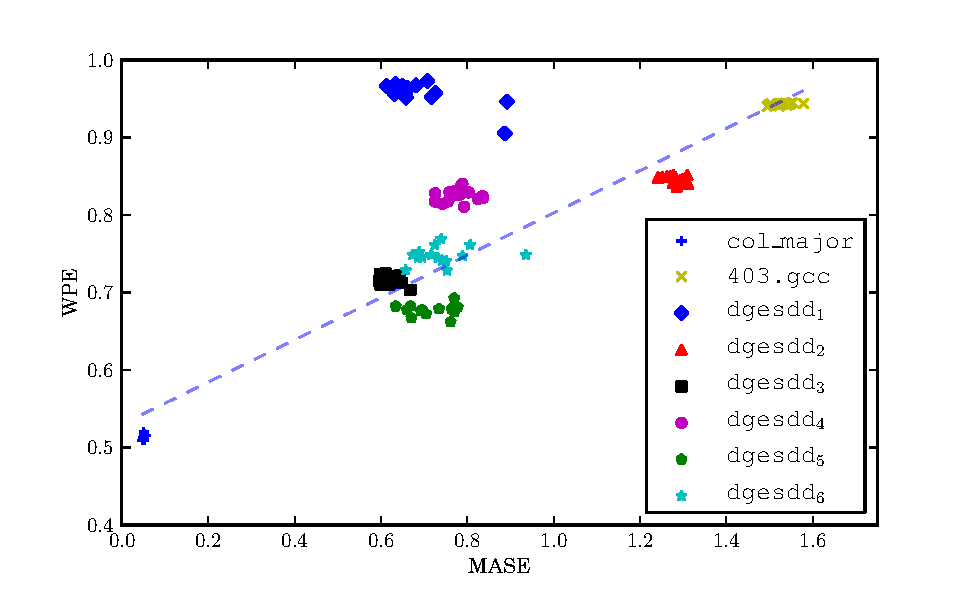
\includegraphics[width=1.1\columnwidth]{figs/new_prediction_vs_entropy}
  \caption{Weighted permutation entropy vs. mean absolute scaled error
    (MASE) of the best prediction of each time series.  The solid
    curve is a least-squares log fit of these points.
%
% of all the points except those from {\tt dgesdd$_1$}, which we have
% excluded for reasons explained in the text.
%
The dashed curves reflect the standard deviation of the model in its
parameter space.  The meaning of the shaded region is explained in the
text.}
  \label{fig:wpe_vs_mase_best}
\end{figure}
%
% As the plot shows, the best-case prediction error for each trace from
% these eight systems is roughly proportional to the log of the weighted
% permutation entropy, which is consistent with our first conjecture.
%
There is an obvious upward trend, which is consistent with the notion
that there is a pattern in the WPE-MASE relationship.  However, a
simple linear fit is a bad idea here.  First, any signal with zero
entropy should be perfectly predictable (i.e., MASE $\approx 0$), so
any curve fitted to these data should pass through the origin.
Moreover, WPE does not grow without bound, so one would expect the
patterns in the WPE-MASE pairs to reach some sort of asymptote.  For
these reasons, we chose to fit a function of the form $y = a \log(b x
+ 1)$ to these points, with $y =$ WPE and $x=$ MASE\footnote{The
  specific values of the coefficiencts are $a=7.97 \times 10^{-2}$ and
  $b=1.52 \times 10^3$.}.  The solid curve in the figure shows this
fit; the dashed curves show the standard deviation of this model in
its parameter space: i.e., $y = a \log(b x + 1)$ with $\pm$ one
standard deviation on each of the two parameters.  Points that fall
within this deviation volume (light grey) correspond to predictions
that are comparable to the best ones found in this study; points that
fall \emph{above} that volume (dark grey) are better still.  We chose
to truncate the shaded region because of a subtle point regarding the
MASE of an ideal predictor, which should not be larger than 1 unless
the training and test signals are different.  This is discussed at
more length below.

The curves and regions in Figure~\ref{fig:wpe_vs_mase_best} are a
graphical representation of the first finding.  This representation
is, we believe, a useful heuristic for determining whether a given
prediction method is well matched to a particular time series.  It is
not, of course, a formal result.  The forecast methods and data sets
used here were chosen to span the space of standard prediction
strategies and the range of dynamical behaviors, but they do not cover
those spaces exhaustively.  Our goal here is an \emph{empirical}
assessment of the relationship between predictability and complexity,
not formal results about a ``best'' predictor for a given time series.
There may be other methods that produce lower MASE values than those
in Figure~\ref{fig:wpe_vs_mase_best}, but the sparseness of the points
above and below the one-$\sigma$ region about the dashed curve in this
plot strongly suggests a pattern of correlation between the underlying
predictability of a time series and its WPE.  The rest of this section
describes these results and claims in more detail---including the
measures taken to assure meaningful comparisons across methods,
trials, and programs---and elaborates on the meaning of the different
curves and limits in the figure.

Figure~\ref{fig:wpe_vs_mase_all} shows WPE vs. MASE plots for the full
set of experiments.
\begin{figure*}
  \centering
%    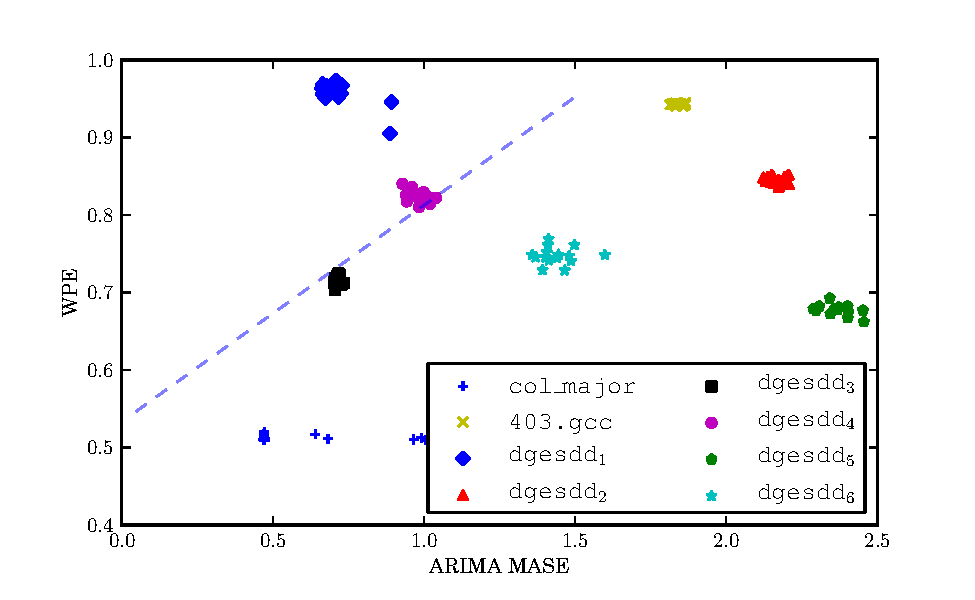
\includegraphics[width=\columnwidth]{figs/ARIMA_prediction_vs_entropy}
%    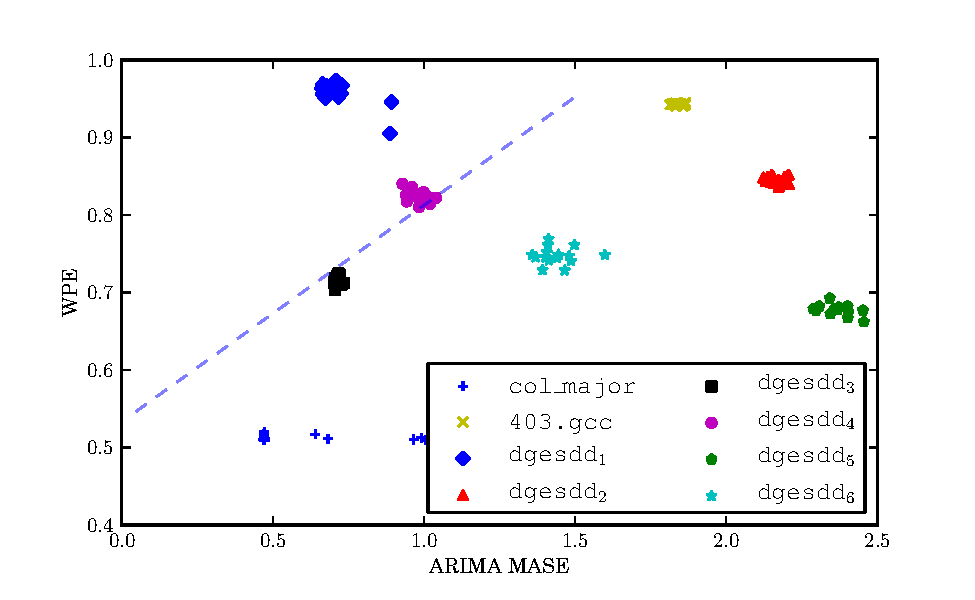
\includegraphics[width=\columnwidth]{figs/ARIMA_prediction_vs_entropy}
%    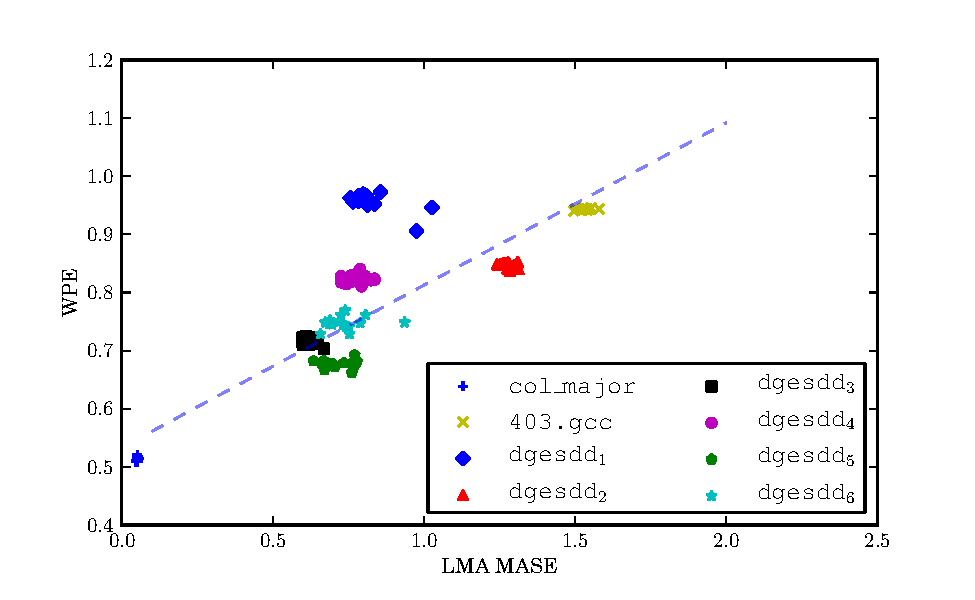
\includegraphics[width=\columnwidth]{figs/LMA_prediction_vs_entropy}
  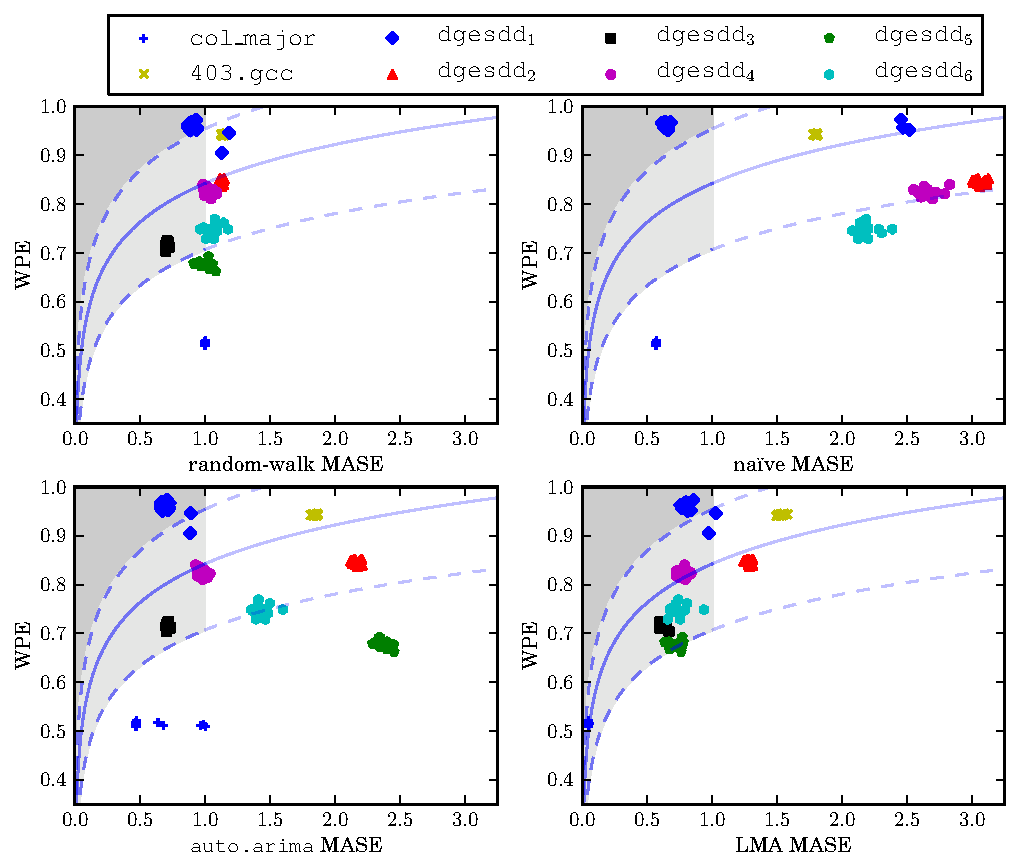
\includegraphics[width=1.7\columnwidth]{figs/new_predictions_vs_entropy4a}
\caption{WPE vs. MASE for all trials, methods, and systems---with the
  exception of \svdone, \svdthree, and \svdfive are omitted from the
  top-right plot for scale reasons, as described in the text.
%
% ; their MASE scores are $2.676 \pm 4.328$, $31.39 \pm 0.282$, and
%   $20.87 \pm 0.192$ respectively.
%
Numerical values, including means and standard deviations of the
errors, can be found in Table~\ref{tab:error}.  The curves and shaded
regions are the same as in the previous figure.  }
    \label{fig:wpe_vs_mase_all}
\end{figure*}
There are 15 points in each cluster, one for each trial.  (The points
in Figure~\ref{fig:wpe_vs_mase_best} are the leftmost of the points
for the corresponding trace in any of the four plots in
Figure~\ref{fig:wpe_vs_mase_all}.)  The WPE values do not vary very
much across trials.  For most traces, the variance in MASE scores is
low as well, resulting in small, tight clusters.  In some
cases---\arima predictions of {\tt col\_major}, for instance---the
MASE variance is larger, which spreads out the clusters horizontally.
The mean MASE scores of predictions generated with the nonlinear LMA
method, for instance, are generally closer to the dashed curve; the
\arima method clusters are more widely spread, the \naive ~clusters
even more so.  A few of the clusters have very high variance; these
are discussed later in this section.

The main thing to note here, however, is not the details of the shapes
of the clusters, but rather their positions in the four plots:
specifically, the fact that many of them are to the right of and/or
below the dashed curve that identifies the boundary of the shaded
region.  \emph{These predictions are not as good as our heuristic
  suggests they could be.}  Focusing in on any single cluster of
points makes this clear: LMA works best for \svdsix, for instance,
followed by the random-walk prediction method, then \arima and \naive.
When a practitioner calculates an WPE vs. MASE value that is outside the
shaded region, that should suggest to her that the prediction method
is not well matched to the task at hand: that is, the time series has
more predictive structure than the method is able to use.
%
% The idea behind the shaded region is to help practitioners identify
% when there is predictive structure in the data that a given method is
% not exploiting (viz., \arima on \svdsix)---i.e., that one could do
% better with another forecast strategy.
%
In this case---e.g., \arima on \svdsix---she should try a different
method.  The position of the LMA cluster for \svdsix, on the other
hand, reflects this method's ability to capture and exploit the
structure that is present in this signal.  WPE vs. MASE values like
this, which fall in the shaded region, should suggest to the
practitioner that the prediction method is well-suited to the task.
The following discussion lays out the details that underlie these
claims.
%
% The dashed curve in Figures~\ref{fig:wpe_vs_mase_best}
% and~\ref{fig:wpe_vs_mase_all} is a heuristic that captures the
% argument at the end of the previous paragraph.
%

Though \col is a very simple program, its dynamics are actually quite
complicated, as discussed in Section~\ref{sec:intro}.  Recall from
Figure~\ref{fig:forecast-example} and Table~\ref{tab:error} that the
\naive, \arima, and (especially) random-walk prediction methods do not
perform very well on this signal.  The MASE scores of these
predictions are $0.571 \pm 0.002$, $1.001 \pm 0.002$, and $0.599 \pm
0.211$, respectively, across all 15 trials.  That is, \naive ~and
\arima are performing only $\approx 1.7$ times better than the
random-walk method, a primitive strategy that simply uses the current
value as the prediction.  However, the WPE value for the \col trials
is $0.513 \pm 0.003$, which is in the center of the complexity
spectrum described in Section~\ref{sec:intro}.

This disparity---WPE values that suggest a high rate of forward
information transfer in the signal, but predictions with comparatively
poor MASE scores---is obvious in the geometry of the two left-hand
and the upper-right hand images in Figure~\ref{fig:wpe_vs_mase_all}, where the \col clusters
are far to the right of and/or below the dashed curve.  Again, this
indicates that these methods are not leveraging the available
information in the signal.  The dynamics of \col may be complicated,
but they are not unstructured.  This signal is nonlinear and
deterministic~\cite{mytkowicz09}, and if one uses a prediction
technique that is based a nonlinear model (LMA)---rather than a method
that simply predicts the running mean (\naive) or the previous value
(random walk), or one that uses a linear model (\arima)---the MASE
score is much better: $0.050 \pm 0.001$.  This prediction is 20 times
more accurate than a random-walk forecast, which is more in line with
the level of predictive structure that the low WPE value suggests is
present in the signal.  The MASE scores of random-walk predictions of
\col are all $\approx 1$---as one would expect---pushing those points
well below the shaded region.  Clearly the stationarity assumption on
which this method is based does not hold for this signal.

Note that the \col points (blue {\color{blue}$+$} icons) are clustered
very tightly in the lower left quadrant of the \naive, random-walk,
and LMA plots in Figure~\ref{fig:wpe_vs_mase_all}, but spread out
horizontally in the \arima plot.  This is because of the way the
\arima process builds ARIMA models \cite{autoARIMA}.  If a KPSS test
of the time series in question indicates that it is nonstationary, the
\arima recipe adds an integration term to the model.  This test gives
mixed results in the case of the \col process, flagging five of the 15
trials as stationary and ten as nonstationary.  ARIMA models without
an integration term perform more poorly on this signal, which
increases the error, thereby spreading out the points.  We tested this
hypothesis by forcing the inclusion of an integration term in the five
cases where a KPSS test indicated that such a term was not needed.
This action removed the spread, pushing all 15 of the \col ~ \arima
points in Figure~\ref{fig:wpe_vs_mase_all} into a tight cluster.
%\alert{Josh to do: this paragraph needs more, in response to the %ref's
%  gritch about fitting: the stuff about \arima being an automated
%  recipe that can give bad results, and the fact that our %technique
%  can tell when it does.  Look at the response letter for context %and
%  ammunition---and also put something in there that calls his
%  attention to this paragraph.}


The discussion in the previous paragraph brings to light an interesting feature of our proposed heuristic. The \arima algorithm that was used to build all of the ARIMA
models in this paper, follows the procedure outlined
in Section V B to choose values for the model parameters.
As discussed previously, this algorithm employs sophisticated tests, such as the KPSS test, to intelligently traverse and reduce model space and then uses well-known criterion for choosing the most-likely of the remaining models. However, it is quite possible that this procedure can choose a sub-optimal fit. Specifically, if the initial space of models being searched is not broad enough, or if one of the preliminary tests gives an erroneous result, then the best ARIMA model may be excluded or eliminated before likelihood is even examined. This circumstance is hard to detect. Maximal-likelihood  tests, such as AIC used in \arima, can only conclude which of the models provided is ``most likely"---but cannot conclude that \emph{none} of the models are likely. In contrast,
%Sometimes the choices made by that procedure produce a sub-optimal predictor, however there is nothing to say whether a different model from the ARIMA class would work better.
inappropriate MASE scores (compared to
what the WPE value might suggest) may suggest an inappropriateness in the order selection and parameter estimation procedure, which would flag to a practitioner to reevaluate the appropriateness of fit. For example,
%During the fitting process of \arima many subclasses of ARIMA models are eliminated based on various tests, such as the KPSS test. If these tests give erroneous results then entire subclasses of ARIMA models are never even considered. Our heuristic may be able to flag when this has occurred.
by examining the \arima MASE scores vs. WPE values of \col, we were able to see that, while all signal complexities were the same, some of the signals had much higher MASE values. This suggested to us inappropriate parameter selection for these time series. We then went back and manually assisted the automated fitting procedure, resulting in models with consistent MASE vs WPE score, and improved forecasts.















The WPE of \svdfive ($0.677 \pm 0.006$) is higher than that of {\tt
  col\_major}.  This indicates that the rate of forward information
transfer of the underlying process is lower, but that time-series data
observed from this system still contain a significant amount of
structure that can, in theory, be used to predict the future course of
the time series.
% As mentioned above, though, the effectiveness of any prediction
% strategy depends on how well it leverages the information that is
% available in the data: methods that use linear models, for instance,
% may fail when applied to nonlinear processes.  (This is the basis
% for the second conjecture above.)
The MASE scores of the \naive ~and \arima predictions for this system
are $20.870 \pm 0.192$ and $2.370 \pm 0.051$, respectively: that is,
20.87 and 2.37 times worse than a simple random walk forecast of the
same signals\footnote{The \naive ~MASE score is large because of the
  bimodal nature of the distribution of the values of the signal,
  which makes guessing the mean a particularly bad strategy.  The same
  thing is true of the \svdthree signal.}.  As before, the positions
of these points on a WPE vs. MASE plot---significantly below and to
the right of the shaded region---should suggest to a practitioner that
%  there is more structure in this signal than the corresponding
% method is able to leverage, and that
a different method might do better.  Indeed, for \svdfive, the LMA
method produces a MASE score of $ 0.718\pm 0.048 $ and a cluster of
results that largely within the shaded region on the WPE-MASE plot.
This is consistent with our second finding: the LMA method can capture
and reproduce the way in which the \svdfive system processes
information, but the \naive ~and \arima prediction methods cannot.

The WPE of \gcc is higher still: $0.943 \pm 0.001$.  This system
transmits very little information forward in time and provides almost
no structure for prediction methods to work with.  Here, the
random-walk predictor is the best of the methods used here.  This
makes sense; in a fully complex signal, where there is no predictive
structure to utilize, methods that depend on exploiting that
structure---like ARIMA and LMA---will be outperformed by methods that
do not rely on that structure.
%
% in a fully complex signal, the MASE of a random-walk forecast will
% always be $\approx 1$, assuming that the training signal accurately
% reflects the overall behavior of the out-of-sample time series
%
Since fitting a hyperplane using least squares should filter out some
of the noise in the signal, the fact that LMA outperforms \arima
($1.530 \pm 0.021$ vs. $1.837 \pm 0.016$) may be somewhat
counterintuitive.  However, the small amount of predictive structure
that is present in this signal is nonlinear (cf.,~\cite{mytkowicz09}),
and LMA is designed to capture and exploit that kind of structure.
Note that all four \gcc clusters in Figure~\ref{fig:wpe_vs_mase_all}
are outside the shaded region; in the case of the random-walk
prediction, for instance, the MASE value is $1.1381 \pm 0.011$.  This
is due to nonstationarity in the signal: in particular, differences
between the training and test signals.  \svdtwo fits the same
patterns, for the same reasons---and visibly so, in the red segment of
Figure~\ref{fig:svd-ts-colored}, where the period and amplitude of the
oscillations are decreasing.

\svdone---the dark blue segment of
Figure~\ref{fig:svd-ts-colored}---behaves very differently than the
other seven systems in this study.  Though its weighted permutation
entropy is very high ($0.957 \pm 0.016$), three of the four prediction
methods do quite well on this signal, yielding mean MASE scores of
0.714 (\arima), 0.827 (LMA), and 0.933 (random walk).  This pushes the
corresponding clusters of points in Figure~\ref{fig:wpe_vs_mase_all}
well above the trend followed by the other seven signals.  The reasons
for this are discussed in the following paragraph.  The MASE scores of
the predictions that were produced by the \naive ~method for this
system, however, are highly inconsistent.  The majority of the blue
diamond-shaped points on the top-right plot in
Figure~\ref{fig:wpe_vs_mase_all} are clustered near a MASE score of
0.6, which is better than the other three methods.  In five of the 15
\svdone trials, however, there were step changes in the signal.  The
\naive ~method has a very difficult time with signals like this,
particularly if there are multiple step changes.  This raised the MASE
scores of these trials, pushing the corresponding points to the
right\footnote{This includes the cluster of three points near MASE
  $\approx 2.5$, as well as two points that are beyond the domain of
  the graph, at MASE $\approx 11.2-14.8$.}, and in turn raising both
the mean and variance of this set of trials.

The effects described in the previous paragraph are also exacerbated
by the way MASE is calculated.  Recall that MASE scores are scaled
\emph{relative to a random-walk forecast of the training set}.  There
are two issues here.  First, random-walk prediction works very badly
on signals with frequent, large, rapid transitions.  Consider a signal
that oscillates from one end of its range to the other at every step.
A signal like this will have a low WPE, much like {\tt col\_major}.
However, a random-walk forecast of this signal will be 180 degrees out
of phase with the true continuation.  Since random-walk error appears
in the denominator of the MASE score, this effect can shift points
leftwards on a WPE vs. MASE plot, and that is exactly why the \svdone
clusters in Figure~\ref{fig:wpe_vs_mase_all} are above the dashed
curve.  This time series, which is shown in closeup in
Figure~\ref{fig:svdone-ts},
\begin{figure}[htbp]
  \centering
    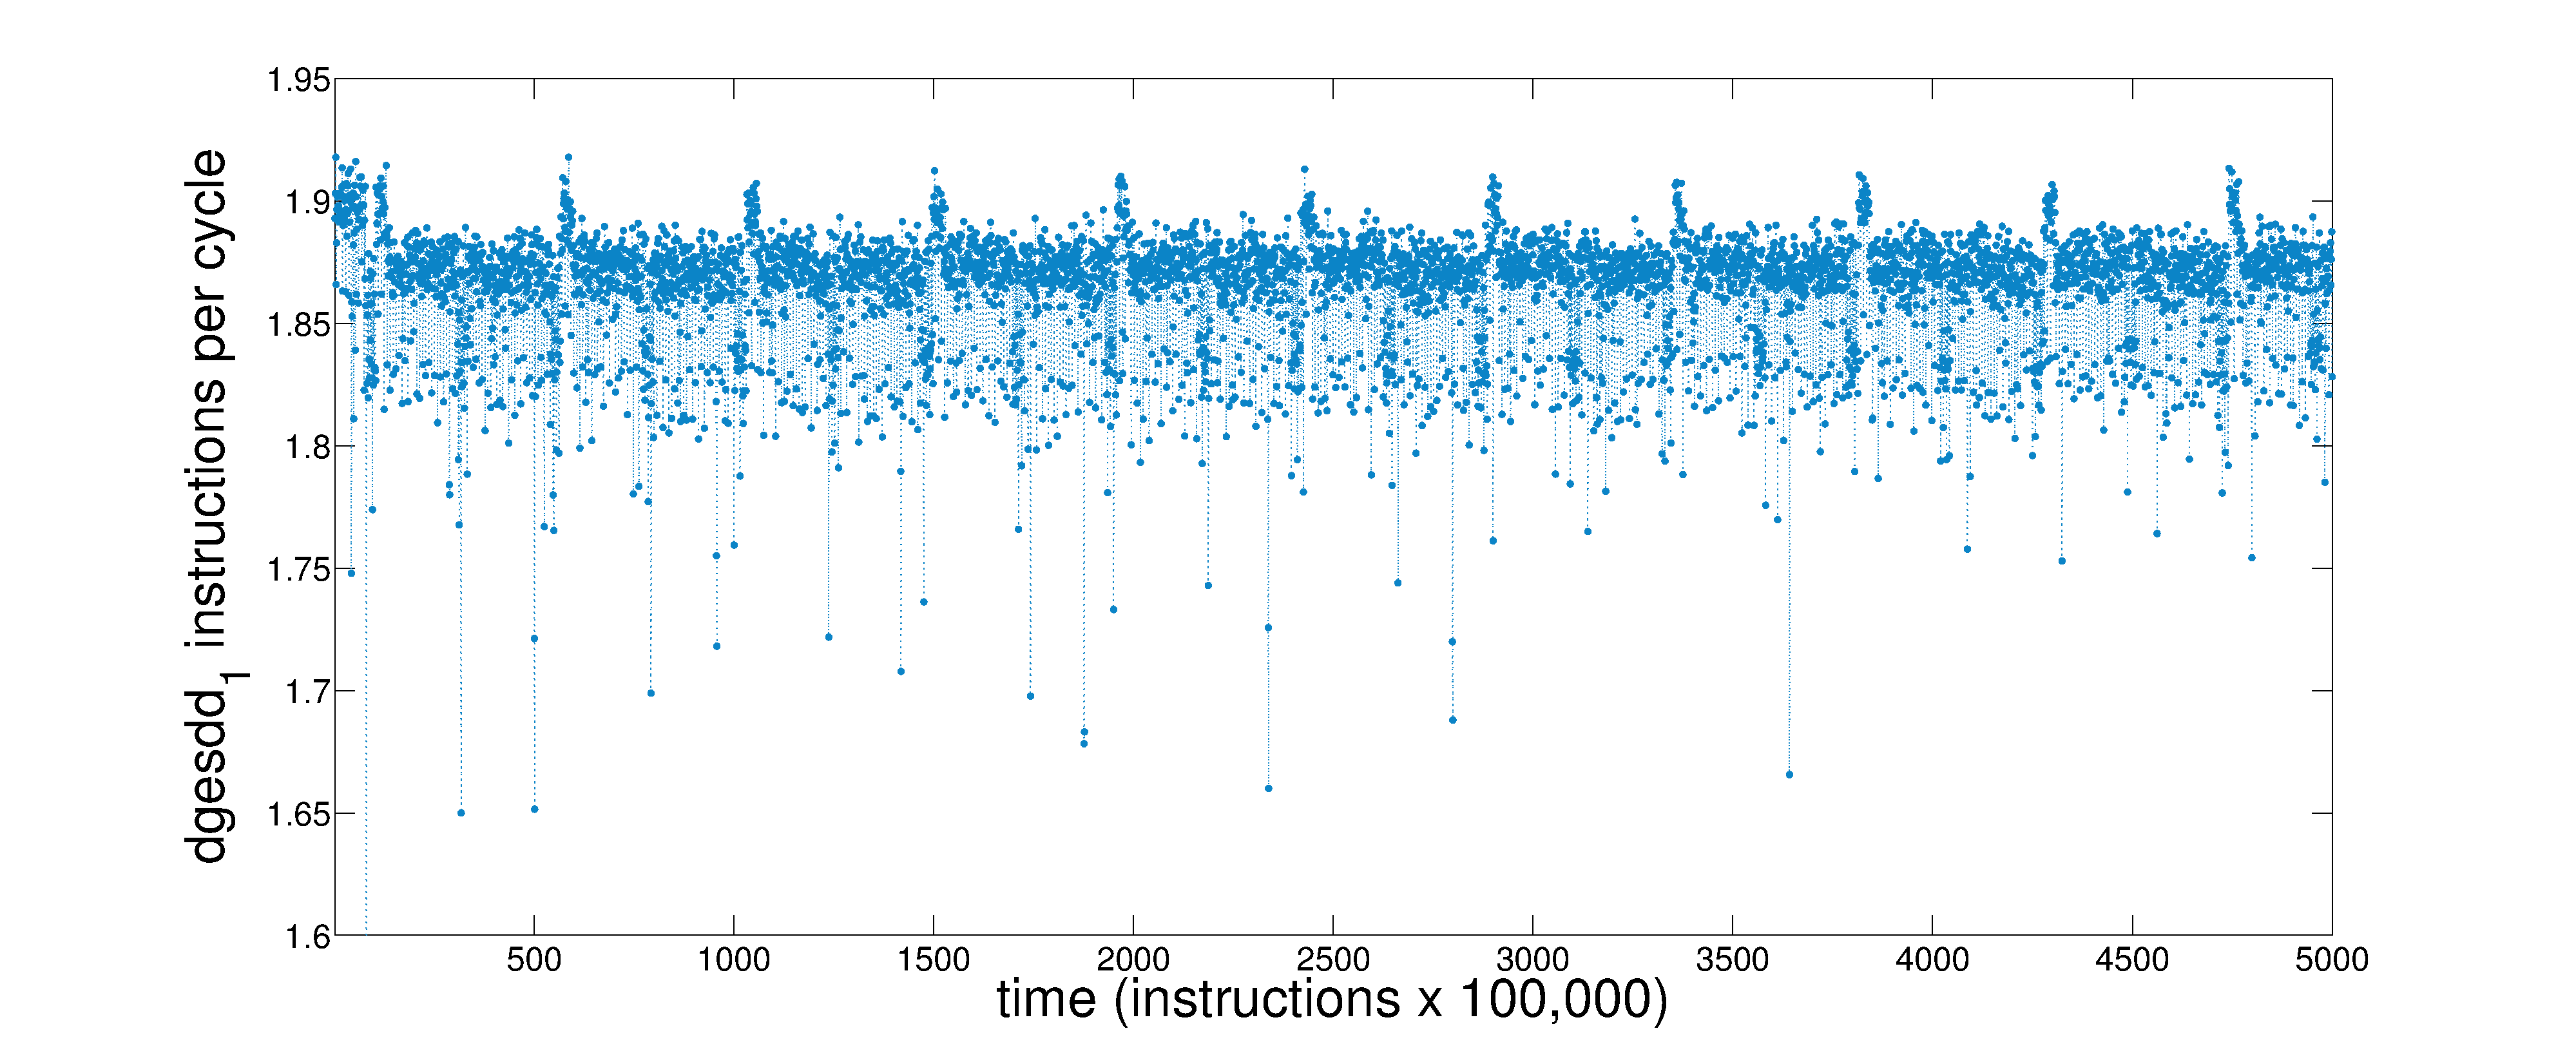
\includegraphics[width=\columnwidth]{figs/svdonets2}
\caption{A small portion of the \svdone time series}\label{fig:svdone-ts}
\end{figure}
is not quite to the level of the worst-case signal described above,
but it still poses a serious challenge to random-walk prediction.  It
is dominated by a noisy regime (between $\approx$1.86 and
$\approx$1.88 on the vertical scale in Figure~\ref{fig:svdone-ts}),
punctuated by short excursions above 1.9.  In the former regime, which
makes up more than 80\% of the signal, there are frequent dips to 1.82
and occasional larger dips below 1.8.  These single-point dips are the
bane of random-walk forecasting.  In this particular case, roughly
40\% of the forecasted points are off by the width of the associated
dip, which skews the associated MASE scores.  Signals like this are
also problematic for the \naive ~prediction strategy, since the
outliers have significant influence on the mean.  This compounds the
effect of the skew in the scaling factor and exacerbates the spread in
the \svdone MASE values.

% For all of these reasons, we view \svdone as an outlier and exclude it
% from the fit calculation of the dashed curve in
% Figure~\ref{fig:wpe_vs_mase_best}.

The second effect that can skew MASE scores is nonstationarity.  Since
this metric is normalized by the error of a random-walk forecast
\emph{on the training signal}, differences between the test signal and
training signal can create issues.  This is why the MASE values in
Table~\ref{tab:error} are not identically one for every random-walk
forecast of every time series: the last 10\% of these signals is
significantly different from the first 90\%.  The deviation from 1.00
will depend on the process---whether it has multiple regimes, what
those regimes look like, and how it switches between them---as well as
the experimental setup (e.g., sensor precision and data length).
Nonetheless, this effect suggests another potentially useful
heuristic: if the MASE of a random-walk prediction of a time series is
significantly different from 1, this could be an indication that the
signal is nonstationary.  \alert{Should we point back to the obvious
  MASE wall in the figure to add weight to this?}  We are in the
process of exploring this idea.

Again, the curves in Figures~\ref{fig:wpe_vs_mase_best}
and~\ref{fig:wpe_vs_mase_all} were determined from a finite set of
methods and data.  We put a lot of thought and effort into making
these experiments upon which these results are based both
representative and comprehensive.  The forecast methods involved range
from the simple to the sophisticated; the time-series data was sampled
from a system whose behavior spans the dynamical behavior space.
While we are cautiously optimistic about the generality of our
conclusions, more exploration will be required before we can make any
such claim.  Our preliminary work along those lines shows that data
from the Henon map \cite{henon}, the Lorenz system \cite{lorenz}, and
the SFI A data set \cite{sfi-data} all fall within the one-$\sigma$
volume of the fit in Figures~\ref{fig:wpe_vs_mase_best}
and~\ref{fig:wpe_vs_mase_all} region, as do various nonlinear
transformations of \svdtwo, \svdfive and \svdsix.

Of course, the geometry of these curves and bounds do not necessarily
extend to other error metrics.  The positions of the WPE vs. error
points---and the reasons to choose a particular function to fit to
them or impute theoretical bounds on the meaning of the results---may
change if one calculates error using a procedure other than the one
described in Section~\ref{sec:accuracy}.  The MASE error metric, as
discussed above, has its weaknesses.  Even so, we concur with
\cite{MASE} that it is an effective way to compare prediction error
across time-series data of different lengths and different scales, and
we are convinced by the extensive evaluations that are offered in that
paper, as well as the comparisons of MASE to other metrics, that its
strengths far outweigh its weaknesses.

%This portion should justify the following claim%%%%%%%%%%%%%%%%%%%%%%
%\item The way structure/information/complexity is processed internally by a given process plays a crucial role in predictability.
%%%%%%%%%%%%%%%%%%%%%%%%%

%In Figures~\ref{fig:lma_pred_vs_ent} and \ref{fig:arima_pred_vs_ent} we directly compare the performance of the LMA and ARIMA prediction methods (respectively) to the value of the weighted permutation entropy for all runs of each program under consideration. The LMA MASE values are largely similar to those of the best predictions, primarily because LMA often performed superior to ARIMA (and the na\"ive method). On the other hand, the ARIMA MASE values are largely uncorrelated with WPE values. As was hinted at while discussing the previous results, the fact that ARIMA is uncorrelated with WPE brings about an interesting perspective on information transfer and WPE. The WPE is sensitive to both linear and nonlinear structure. When you have a low WPE and a high ARIMA it could be that the structure WPE is picking up is simply nonlinear structure that LMA can handle but ARIMA cannot. So while ARIMA is consistently out performed by random walk,  there is plenty of structure present as suggested by WPE and taken advantage of by LMA but since it is nonlinear ARIMA can't take it into account and does bad.



%is in large part one of the major findings of this work. More specifically, say we tried to predict an arbitrary noisy real-valued time series with an ``out-of-the-box" prediction strategy like ARIMA as proposed in \cite{autoArima} and say we got inconsistent and bad forecasts, (i.e., perform worse than the na\"ive random walk strategy ($MAS>1$). How do we determine if the prediction strategy is not adequate for the prediction task, or if the signal is simply too complex to predict. If a signal is too complex and too little forward information transfer is present we may not be able to do better than the random walk, in which case we should not worry ourselves over finding a more complicated prediction strategy. However, if we measure the complexity to be low, $\textrm{WPE}<0.85$ (see Fig.~\ref{fig:pred_vs_wpe}) we can most likely do much better than the random walk and should search for more adequate prediction strategies.


